\documentclass[conference]{IEEEtran}
\IEEEoverridecommandlockouts
% The preceding line is only needed to identify funding in the first footnote. If that is unneeded, please comment it out.
%\usepackage{cite}
\usepackage{amsmath,amssymb,amsfonts}
\usepackage{algorithmic}
\usepackage{graphicx}
\usepackage{textcomp}
\usepackage{xcolor}
%\def\BibTeX{{\rm B\kern-.05em{\sc i\kern-.025em b}\kern-.08em
%		T\kern-.1667em\lower.7ex\hbox{E}\kern-.125emX}}


\usepackage{biblatex} 
\addbibresource{refs.bib}

\begin{document}
	
	\title{Analysis on Debris Detection and Trajectory Predictions*}

	\author{\IEEEauthorblockN{1\textsuperscript{st} Yvette Espinoza}
		\IEEEauthorblockA{\textit{Software Engineer} \\
			\textit{Northrop Grumman}\\
			Redondo Beach, CA, USA \\
			yespinoz@purdue.edu}
	}

	\maketitle
	
	\begin{abstract}
		
		Technological improvements over the past few decades have made space exploration more feasible, but the increase in space activity has also resulted in undesirable space debris that can pose a threat to the safety of space crafts. 
		Space surveillance systems can detect and track large debris, providing space situational awareness that reduces the risk of equipment colliding with debris, but such systems often fail to properly identify smaller debris. The main challenge lies with the uncertainty regarding the debris characteristics, making it difficult to accurately predict the orbit.
		Current detection and tracking of small debris is performed by either using ground based systems, or small satellite constellations to gather information on the debris' characteristics and generate orbit predictions.
		This research project will first look at the differences between the two systems, focusing on why small satellite constellations are preferred when considering collision avoidance and active debris removal systems. The iterative closest point algorithm will be discussed as a possible solution to pose estimation, followed by a simulation on how to algorithm works.
		
		% YVETTE - review this again... mention TM and PCA ...?

	\end{abstract}

	\section{Literature Review}
	
		Space exploration, first started in the late 1950's with the USSR's launch of Sputnik I, has become a vital part in current technologies.
		Civilians and government alike have come to rely on space systems, such as GNSS or weather satellites, but the addition of new satellites in an already crowded area is increasing the risk of collisions. 
		This idea was first introduced in 1978 by Kessler, who explained the high density of objects in low Earth orbit (LEO) increases the risk of collisions, and collisions themselves would create more debris that would further increase the collision risk, a scenario commonly referred to as the Kessler Syndrome.
		This scenario was brought back to attention in 2009 with the first recorded collision between between two satellites, Iridium 33 and Cosmos 2251, which at the time produced 1,632 space debris fragments larger than 10 cm \cite{Wang2010AnalysisOD}. These fragments are large enough to be tracked by surveillance systems, such as the Department of Defense’s Space Surveillance Network (SSN), but smaller fragments, referred to as small space debris, are more difficult to detect and track. 
		
		Surveillance networks are catalogs that contain characteristics of registered objects, such as the orbital parameters, which are essential for providing space situational awareness (SSA) \cite{2019_lidar}.
		They rely on both ground based radars and optical telescopes to track the position of the object over time, information that is needed to determine and predict orbits.
		However, applications such as debris collision warning, or active debris removal require information on smaller debris, along with a higher accuracy in orbit determination and prediction, both of which SSN's struggle to provide \cite{2020_ml_approach}.
		
	
	\subsection{Small Satellite Constellations}
		In an effort to increase the accuracy of space debris orbit detection and predictions, studies were conducted to validate the concept of space based space surveillance. In 1996 the Midcourse Space Experiment satellite was launched with a Space-Based Visible (SBV) sensor, becoming the first demonstration of space-based surveillance that could be valuable to the SSN as an addition to the ground based systems \cite{stokes2000space}. In the following years more satellites, such as the SBSS Block 10 and the Sapphire, have been deployed and shown to provide a more accurate description of the environment  \cite{multi_spacecraft_2016}. 
		Onboard sensors have an unobstructed view of debris, not affected by the weather as optical systems are, and can provide more accurate measurements when processing occurs onboard the spacecraft instead of relying on ground control centers.
		
		% YVETTE - more info is needed here... more advantages to using small sattelite constelations
		
		
	\subsection{Pose Acquisition and Tracking}
		One method for onboard pose determination and tracking of space debris involves using a model-based algorithm that processes 3-D point clouds collected from a LIDAR sensor \cite{2017_pose_pca}\cite{liu2016point}\cite{unscented_kalman}.
		The first step is to obtain an initial pose, then refine the pose measurement as part of the tracking and orbit estimation. 
		For the initial pose $p_0 = (\alpha_0, \beta_0, \gamma_0, T_0)$, \cite{2017_pose_pca} proposed a three step method to estimate the relative position vector directly from the measured point cloud, referred to as 3-D PCA-based online Template Matching.
		
		First, the initial position vector ($T_0$) of the satellite with respect to the target, or debris to track, is computed as the centroid of the point cloud. Then the main axes ($e_m$) are estimated using the Principle Component Analysis, where the directions are given by the eigenvectors of the data's covariance matrix ($Q$). The main axes equations are shown in (\ref{eqn:estimated_axes}), while the roll ($\alpha_0$) and pitch ($\beta_0$) estimates are in (\ref{eqn:estimated_roll_pitch}).
		
		\begin{figure}[htbp]
			\centerline{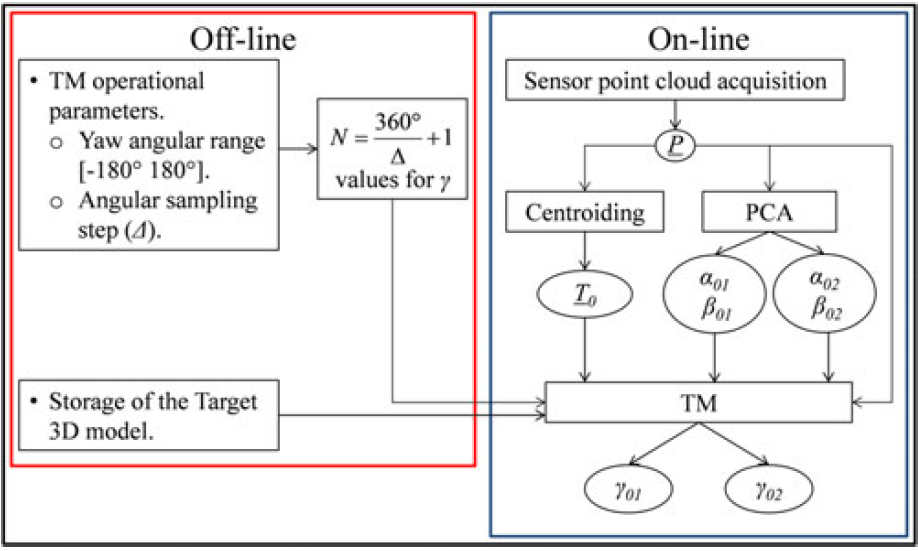
\includegraphics{Images/3_D_PCA_based_TM_algorithm.PNG}}
			\caption{3-D PCA-based online TM algorithm.}
			\label{3_D_PCA_based_TM_algorithm}
		\end{figure}
		
		\begin{equation}
			\label{eqn:estimated_axes}
			\begin{bmatrix} e_{M_x} \\ e_{M_y} \\ e_{M_z} \end{bmatrix}
			=
			\begin{bmatrix}
				cos(\beta_0)  & 0 & -sin(\beta_0) \\
				sin(\alpha_0)sin(\beta_0) & cos(\alpha_0) & sin(\alpha_0)cos(\beta_0) \\
				cos(\alpha_0)sin(\beta_0) & -sin(\alpha_0) & cos(\alpha_0)cos(\beta_0)
			\end{bmatrix}
			\begin{bmatrix} 0 \\ 0 \\ 1 \end{bmatrix}
		\end{equation}
		
		\begin{equation}
			\label{eqn:estimated_roll_pitch}
			\begin{cases}
				\alpha_0 = tan^{-1}(\frac{e_{M_x}}{e_{M_z}}) \\
				\beta_0 = sin^{-1}(-e_Mx)
			\end{cases} 
		\end{equation}
		
		% YVETTE - type out the covarriance matrix along with equation for calculating the centroid!
		
		An overview of the model from acquisition of the point cloud data to the inital pose estimation, taken from \cite{2017_pose_pca} is shown in Figure \ref{3_D_PCA_based_TM_algorithm}.

	\section{Simulation Environment}
		The simulated environment, which takes a known 3-D model and simulates LIDAR point cloud data that would be collected from an orbiting satellite, is generated from \cite{liu2016point}.
		
	\subsection{Target Model}
		Envisat, launched by the European Space Agency in 2002, was selected as the target model because of its large size and relatively simple shape. The satellite, which is 26 m (85 ft) × 10 m (33 ft) × 5 m (16 ft) in orbit, was decommissioned and marked as debris after it lost communication in 2012 \cite{envisat_overview}. A 3-D model was obtained from \cite{envisat_3d_model}, then converted to point cloud data.
		
		% YVETTE - add images of refernce frames and transformations defined
		
		% YVETTE - add image of point cloud data and description showing the image
	
	\subsection{Simulated LIDAR Data}
		
		
	\nocite{*}
	\printbibliography
	
\end{document}
